\section{Results}

All testbenches are implemented as selftesting testsbenches. They contain 
asserts which verify that the expected output has been generated. For the 
low level components the tests are implemented as simple signal assignments 
and assertions. Integration tests are written at the toplevel, here small 
testprograms are loaded into the instruction memory with test data loaded
into data memory, the processor is then enabled for a while. Finally the 
resulting memory state is checked using assert functions.

The test benches are presented in a bottom-up order, and a screenshot is 
provided per testbench. For the higher level 
units or units which contains states, the screenshot is included in the report
and the result is described in more detail. The lower level tests have their test bench results combined into an attached .zip-file, and can be used for easy verification that all assertions pass.



\subsection{Hazard Unit}

The test bench for the hazard unit ensures that the stall and flush signal is asserted when the input is as described in section \ref{sec:hazard_unit}. A screenshot of the test bench executed in Modelsim is included the attachments.


\subsection{Branch Prediction}

The branch prediction test bench verifies that the branch prediction unit uses it internal table to store and predict branches. Figure \ref{fig:branch_prediction_tb} shows what happens to the prediction table if a branch which is in state TAKEN\_STRONG and the branch address is not taken three times in a row.

\begin{figure}[h]
        \centerline{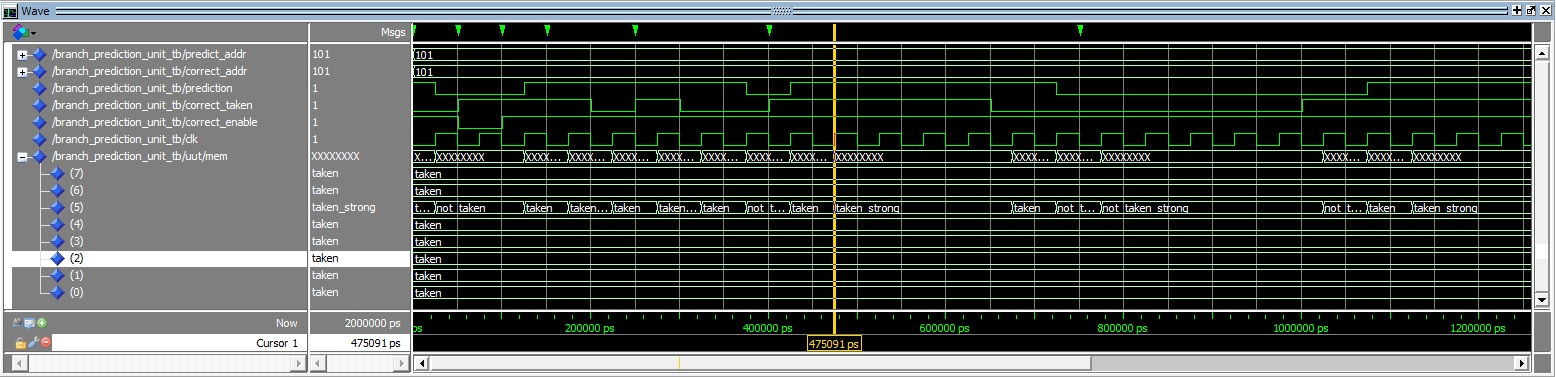
\includegraphics[width=600px]{figures/tb/branch_prediction.jpg}}
        \caption{The branch\_prediction test bench}
        \label{fig:branch_prediction_tb}
\end{figure}
\FloatBarrier

Here the branch address is constanlty 5 and the branch is simulated to repeatedly be not taken, by deasserting the \emph{correct\_taken} signal for four consecutive cycles. From the yellow marker the memory location 5 in the branch unit takes the states TAKEN\_STRONG, TAKEN, NOT\_TAKEN and NOT\_TAKEN\_STRONG. This proves that the branch prediction unit updates it table correctly. By observing the prediction made in the same time period which is high for the states TAKEN\_STRONG and TAKEN and transitions to low when the state changes to NOT\_TAKEN and stays there for the NOT\_TAKEN\_STRONG state.

\subsection{Forwarding Unit} 

This unit checks the registers used in the memory, execute, instruction decode and write back stages and asserts the four forwarding signals A, B, C, D. In the test bench different combinations of the registers are set up and the outputs are asserted. A screenshot of the execution is attached.
\subsection{Next Program Counter Stage}
The pc next stage has four simple cases that are tested. These are tested by setting the inputs correctly and asserting that the output is as expected. The results attached shows that all assertions passes.

\subsection{Instruction Decode Stage}
The instruction decode test bench is divided in two parts. One synchronous part testing the signals going through the register file (this unit is the only synchronous unit in this stage), and one asynchronous part testing the rest of the components. The results of test bench is attached with the other results.

\subsection{Execute Stage}

The execute stage includes the ALU. This unit was included in the assignment startup code and is not tested comprehensivly. But the forwarding logic contained in this stage is. The test bench is selftesting and a screenshot of its execution in Modelsim is included as a attachment.

\subsection{Write Back Stage}

The write back stage test bench is a short test bench which verifies that the write back stage multiplexes the signals correclty and forwards the control signals back to the instruction decode stage. The test is self testing and a screenshot is attached.
\subsection{High level test benches}

The toplevel implementation has four test benches verifying its behaviour.
Like the other test cases these tests are self testing, but a passing test only 
indicates that the result is correct, not that the method of getting there was. 
Hence these tests are harder to verify and are described more in
detail in the following sections. For all the tests a small program is loaded 
into the instruction memory with data loaded into the data memory before the 
processor is enabled for a period of time. 

\subsubsection{Toplevel}
This test bench implements a small, simple program which executes loads, stores, 
adds, ors and ends with a beq instruction which results in a infinite loop.
This test shows the use of most of the implemented instructions, and is quite
large. At the same time it is easy to follow, and we therefore refer the reader
to the screenshot in the attached archive aswell as the actual test bench implementation.

\subsubsection{Branch} 
\label{section:branch-tb}
The branch test bench loads two values into registers and performes four 
conscutive adds. The adds have a data dependecy on the loaded values so the 
first add instruction stalls.
This can be seen when the stall signal goes high in cycle four of figure \ref{fig:branch_tb}.
\begin{figure}[h]
        \centerline{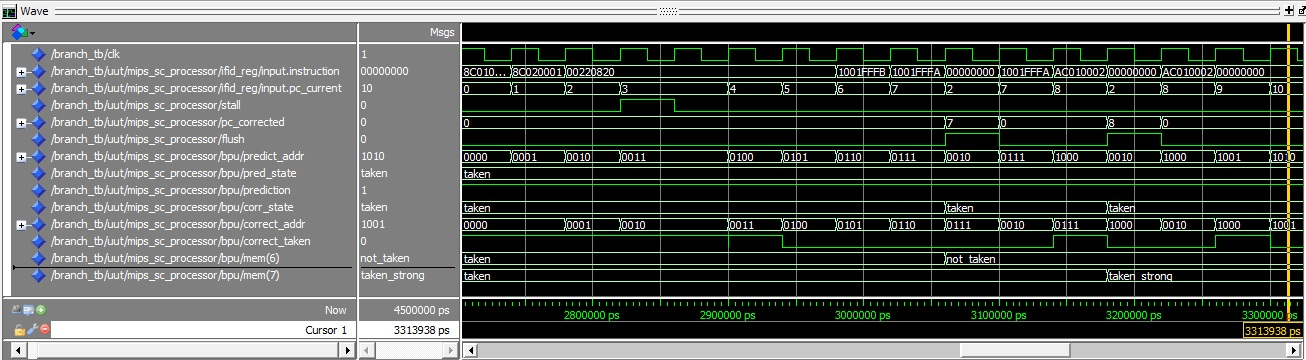
\includegraphics[width=600px]{figures/tb/branch}}
        \caption{The branch test bench}
        \label{fig:branch_tb}
\end{figure}
\FloatBarrier
In cycle 8 (when the \emph{pc\_current} signal is 6) the first branch is fetched from
instruction memory. In the next cycle the second branch is loaded into fetch,
but the branch prediction unit predicts the first branch loaded to be taken. 
As a result the flush signal is pulled high in cycle 9, and the pc changes to
2 in cycle 10.
During cycle 10 the first branch reaches execute, and it is detected that the
branch prediction was wrong. This could have been seen by the correction flush
signal being pulled high, but sadly this signal is missing in the screenshot.
At cycle 11 we're back to instruction 7, the second branch. 

This time the BPU also predicts taken, as seen by the flush. And by cycle 13 
the pc is back to 2. The second branch which now is in execute is evaluated,
and again the prediction was wrong. And in cycle 14 the 8th and final instruction
is loaded.

As mentioned earlier our BPU uses a learning algorithm. The two states for
the two tested branches are shown in the figure. After learning that the first
branch was to be skipped the state changes from TAKEN to NOT\_TAKEN as expected.
However, after the second branch has been evaluated its state changes to TAKEN\_STRONG,
which is wrong. We would expect both of them to end in state NOT\_TAKEN. 
This is caused by a bug in the prediction logic that was not fixed before the deadline.
The bug is not fatal however, as it will only cause some predictions to be sub-optimal.

\subsubsection{For} 
\label{section:for-tb}
This test bench program is a simple for loop, which loops from 1 to 5 before 5 is
written to the data memory. The three constants start, increment and limit are 
initially loaded from data memory.
The loop consists of a branch equal, a add and finally a jump. For each jump taken we
have to flush the if stage, as can be seen by the flush flag. The first time the branch
is evaluated it is predicted taken, as this is the default prediction. But after that one
time it is always predicted not taken, as can be seen by the predict taken signal. During
the last loop the branch is predicted not taken but in fact it should have been taken.
This can be seen by the correction flush close to the end, which clears the IF and ID stages.

This test is a perfect test for our branch predictor as well as forwarding and hazard units
as there are multiple branches, jumps and data hazards. In addition
this testcase is a perfect program to use as a comparison between our two MIPS
implementations. In figures~\ref{fig:for_tb} and ~\ref{fig:multi_cycle_for_tb}, the test output of the test run on both our architectures is shown.

\begin{figure}[h]
        \centerline{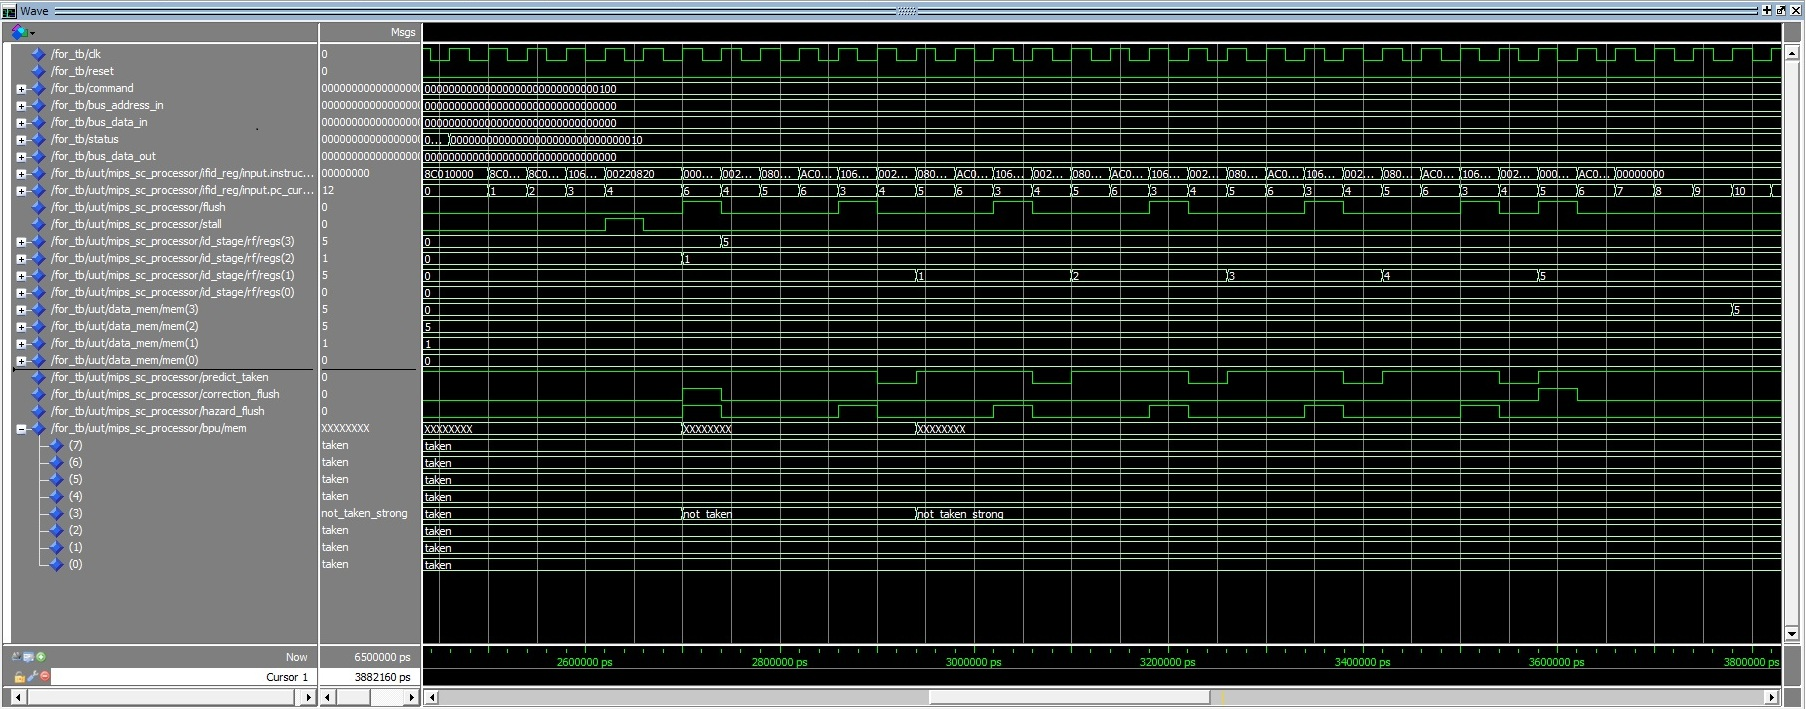
\includegraphics[width=590px]{figures/tb/for_tb2}}
        \caption{For test on pipelined implementation}
        \label{fig:for_tb}
\end{figure}

\begin{figure}[h]
        \centerline{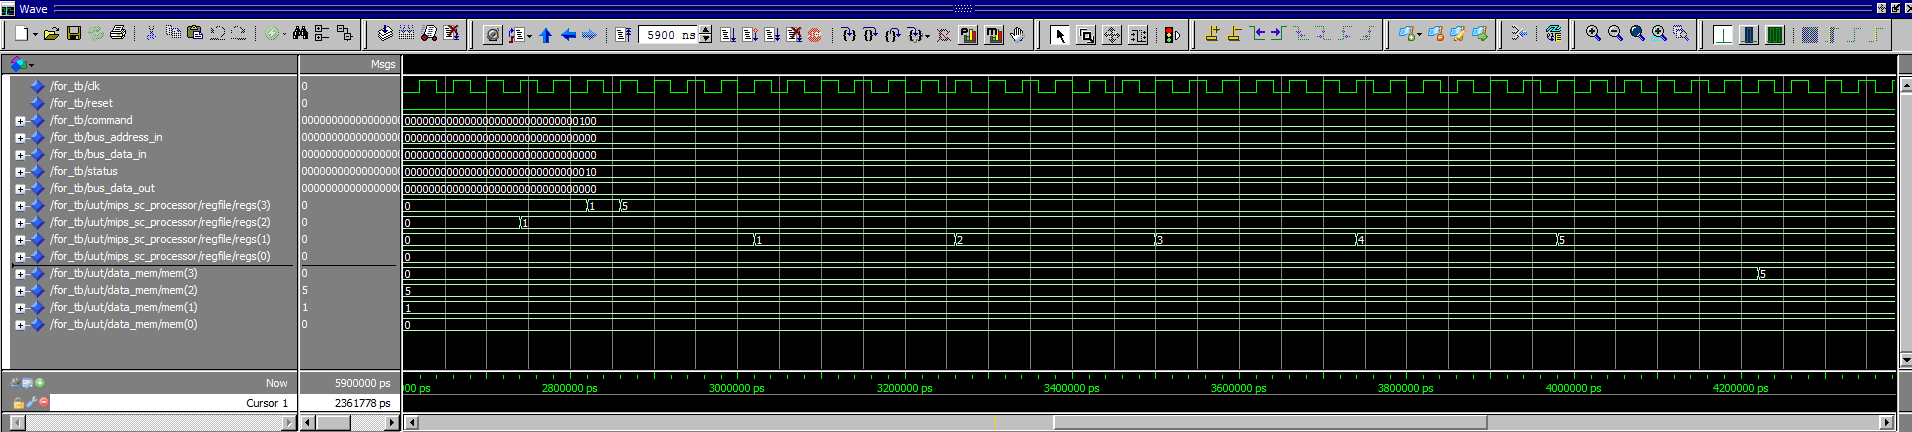
\includegraphics[width=590px]{figures/tb/multicycle_for_test}}
        \caption{For test on multicycle implementation}
        \label{fig:multi_cycle_for_tb}
\end{figure}

As can be read from the two test bench screenshoots, the multicyle
design needs 44 cycles to complete the test while the pipelined design only needs
33 cycles (from the first instruction starts until data is available in memory). 
\FloatBarrier
\FloatBarrier
\section{Implementation on the FPGA}

\subsection{Creating the bit file}
The final bit file {\bf system\_final.bit} is included as a deliverable for easy testing of the project on a FPGA. But the file can also easily be created by following these steps.


\begin{enumerate}
	\item Open the ISE project located at:
		{\bf system/system.xise}
	\item Select the System file in the navigator
  \item Right click on ``Update Bitstream with Processor Data`` and select ReRun All. This process takes a few minutes. 
	\item The result is a file called {\bf system\_download.bit}
\end{enumerate}


\subsection{Uploading the code to the FPGA}
Using the AvProg application installed on the lab, the FPGA can be configured with the {\bf system\_download.bit} or {\bf system\_final.bit} file.
This is done by:

\begin{enumerate}
\item Opening the application and connecting to the Development board through the COM port.
\item Selecting the {\bf .bit} file through the {\bf browse} dialog. 
\item Pressing the {\bf Configure FPGA} button.
\item Disconnecting the COM port. 
\end{enumerate}  

\subsection{Running code on the FPGA}
After the FPGA is configured with the core the {\bf driver/host.py} program can be used to run programs.

To run the {\bf toplevel\_test.hex} program, execute the following commands from the root directory of the project.

Note 1: The -p 3 switch must correspont to the COM port of the test pc. Refere to python driver/host.py -h

Note 2: Because of a late bug the first instruction in the program is not executed. To work around this a {\bf nop} instruction 
is added at the start of the program

\begin{verbatim}
python driver/host.py -p 3 -i ./bin/toplevel_test_nop.hex
python driver/host.py -p 3 -c d 0x1 0x2
python driver/host.py -p 3 -c d 0x2 0xa
python driver/host.py -p 3 -c s
-- wait some time
python driver/host.py -p 3 -c s
python driver/host.py -p 3 -r mem.out
\end{verbatim}

\subsection{Result from running the program}
As in the \ref{sec:exp_res} section the expected output of the program {\bf toplevel\_test.hex} is as per table \ref{table:exp_res}.
The following file snippet shows the result from running the program on the FPGA.

\begin{verbatim}
0x0 0x0
0x1 0x2
0x2 0xa
0x3 0x0
0x4 0x0
0x5 0xc
0x6 0xc
0x7 0xc
0x8 0x600000
0x9 0x713212
0xa	0x0
\end{verbatim}
